\documentclass[12pt]{article}
\usepackage{graphicx}
\setlength{\topmargin}{-.5in}
\setlength{\textheight}{9in}
\setlength{\oddsidemargin}{.125in}
\setlength{\textwidth}{6.25in}
\begin{document}
\title{GINsim tutorial}
\author{Rustin McNeill}
\maketitle

This example will use 2 nodes, one of which is boolean and one of which has three possible 
states. We define the phase space of our system to be as follows:

\begin{center}
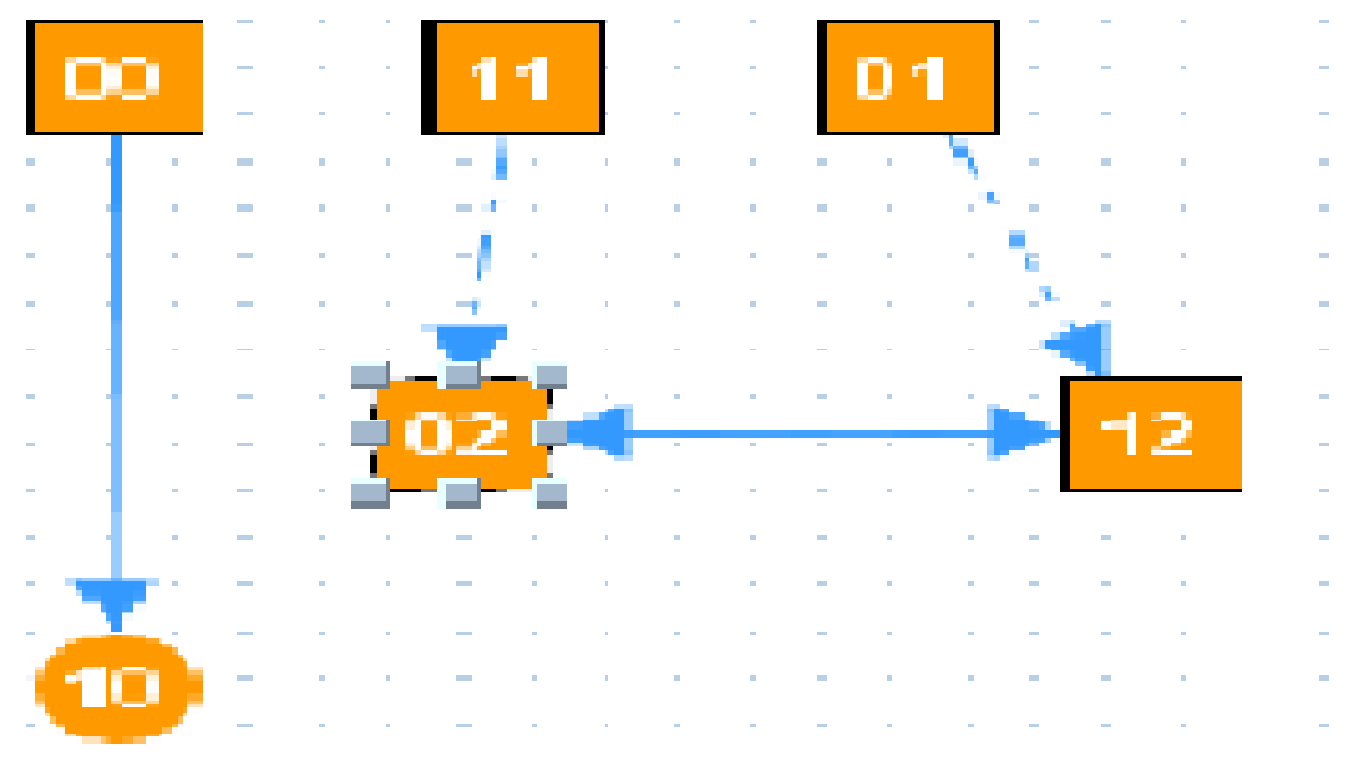
\includegraphics[scale=.15]{2x3ss.png}
\end{center}



We can then make a truth table for each function that assigns a value to the associated index 
given the 2 inputs of a state. 

\begin{table}[ht]
\begin{minipage}[b]{0.5\linewidth}\centering
\begin{tabular}{|c|ccc}
	
$x_{1}$ & & $x_{2}$ \\
	\hline
 $f_{1}$& 0 & 1 & 2  \\
	\hline
0 & 1 & 1 & 1 \\
1 & 1 & 0 & 0 \\
	\hline
\end{tabular}
\end{minipage}
\hspace{0.5cm}
\begin{minipage}[b]{0.5\linewidth}
\centering
 
\begin{tabular}{|c|ccc}
	\hline
$x_{1}$ & & $x_{2}$ \\
	\hline
 $f_{2}$& 0 & 1 & 2  \\
	\hline
0 & 0 & 2 & 2 \\
1 & 0 & 2 & 2 \\
	\hline
\end{tabular}
\end{minipage}
\end{table}
After truth tables have been made for the two functions, we 
can convert this information into a polynomial dynamical system. The functions to this system 
are:
$$f_{1} = x_{1}^{2}x_{2}^{2}+x_{1}x_{2}^{2}+x_{1}^{2}-x_{1}+1$$
$$f_{2} = -x_{1}^{2}x_{2}^{2}+x_{1}x_{2}^{2}-x_{2}^{2}$$
We can compare these functions and their associated state space with the output of ADAM to 
ensure accuracy. To do this we will need to construct a logical model in GINsim. Create two 
nodes in GINsim (you may name them x1 and x2).
\begin{center}
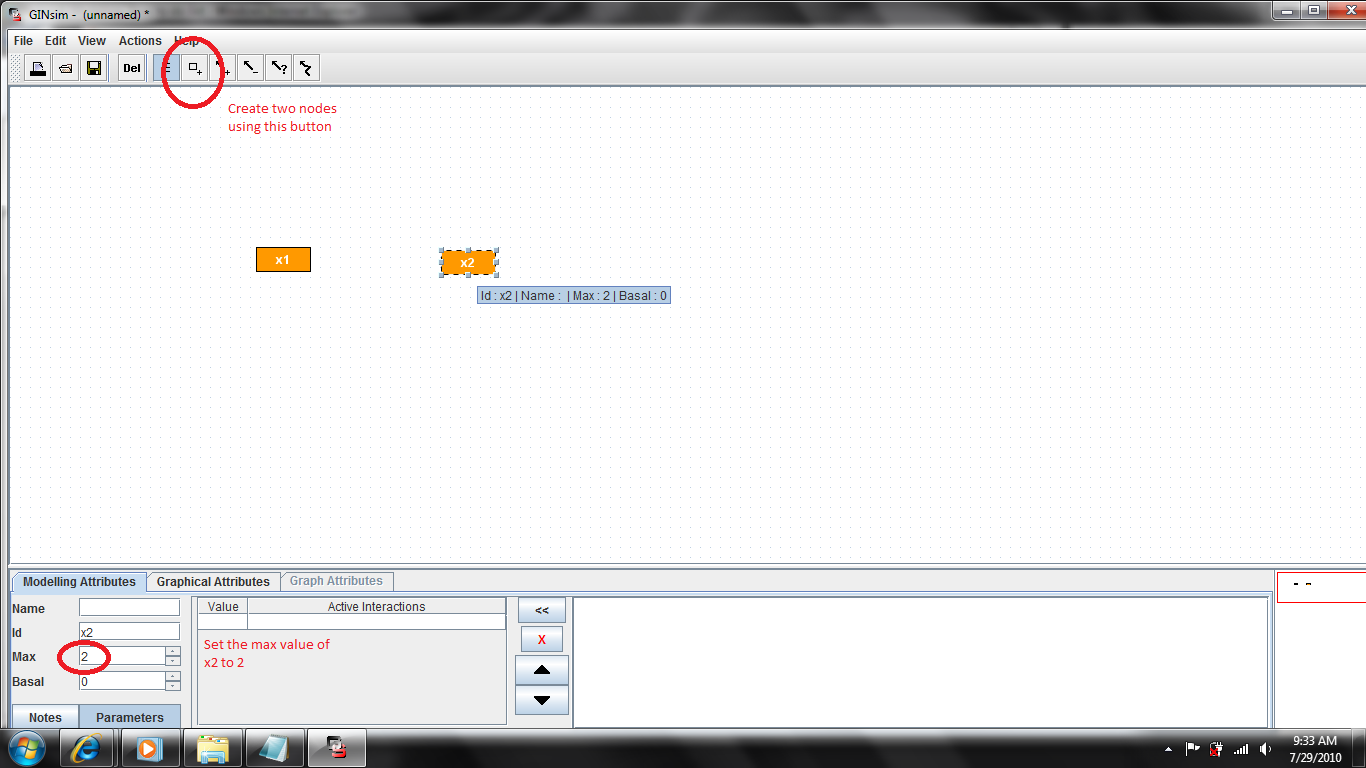
\includegraphics[scale=.43]{createnodes.png}
\end{center}
 Draw edges so that each node has a directed 
edge to the other node, and draw a self loop edge for each node. This is because each node is 
influencing the other node, and itself.

\begin{center}
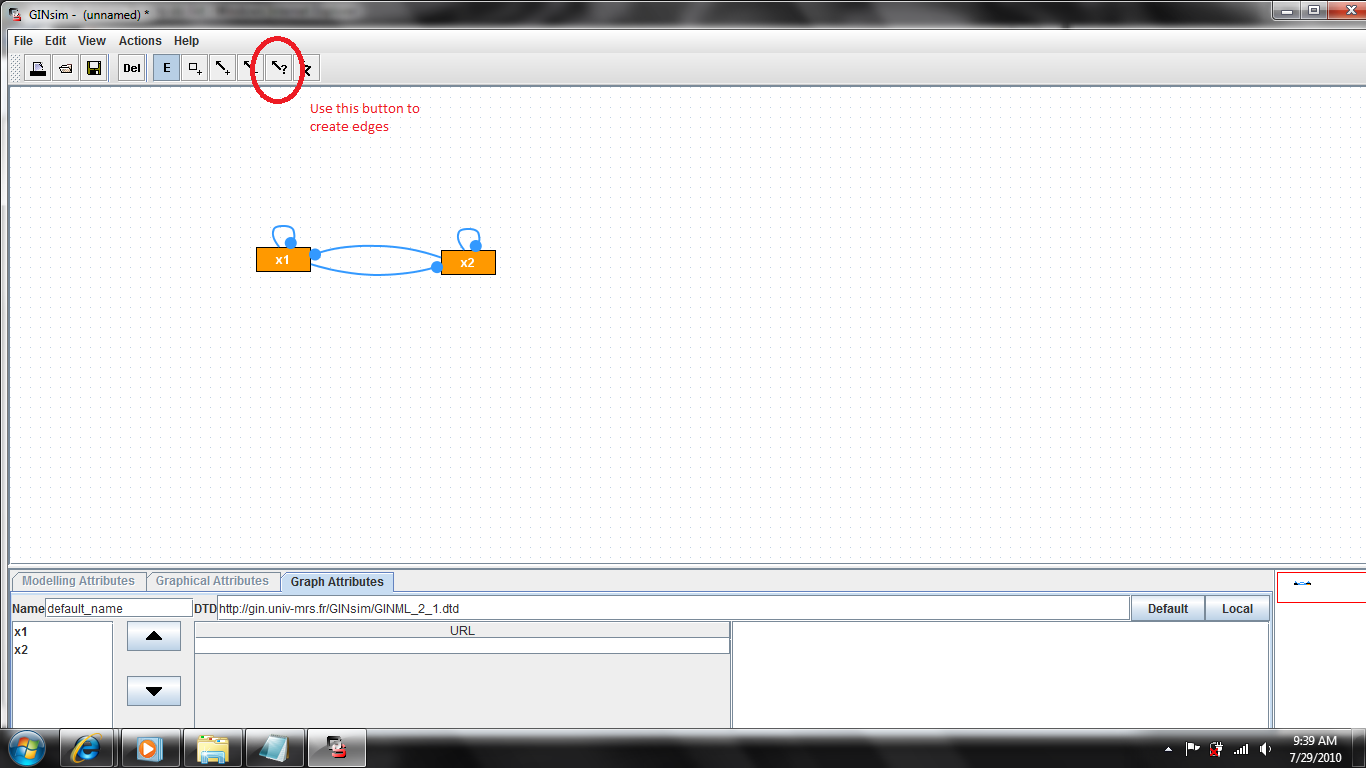
\includegraphics[scale=.43]{createedges.png}
\end{center}

 As x2 is the node with three possible states, for 
each outgoing edge (including the self loop) set x2\_0 as $[1,1]$. This will be used for non-
zero parameters that have x2 as 1. Then set x1 as $[2,2]$, which will be used in non-zero 
parameters that have x2 as 2. As x1 is boolean, leave x1\_0 as $[1,max]$ on all outgoing edges 
from x1 and x2 as 1 is the only nonzero value possible.

\begin{center}
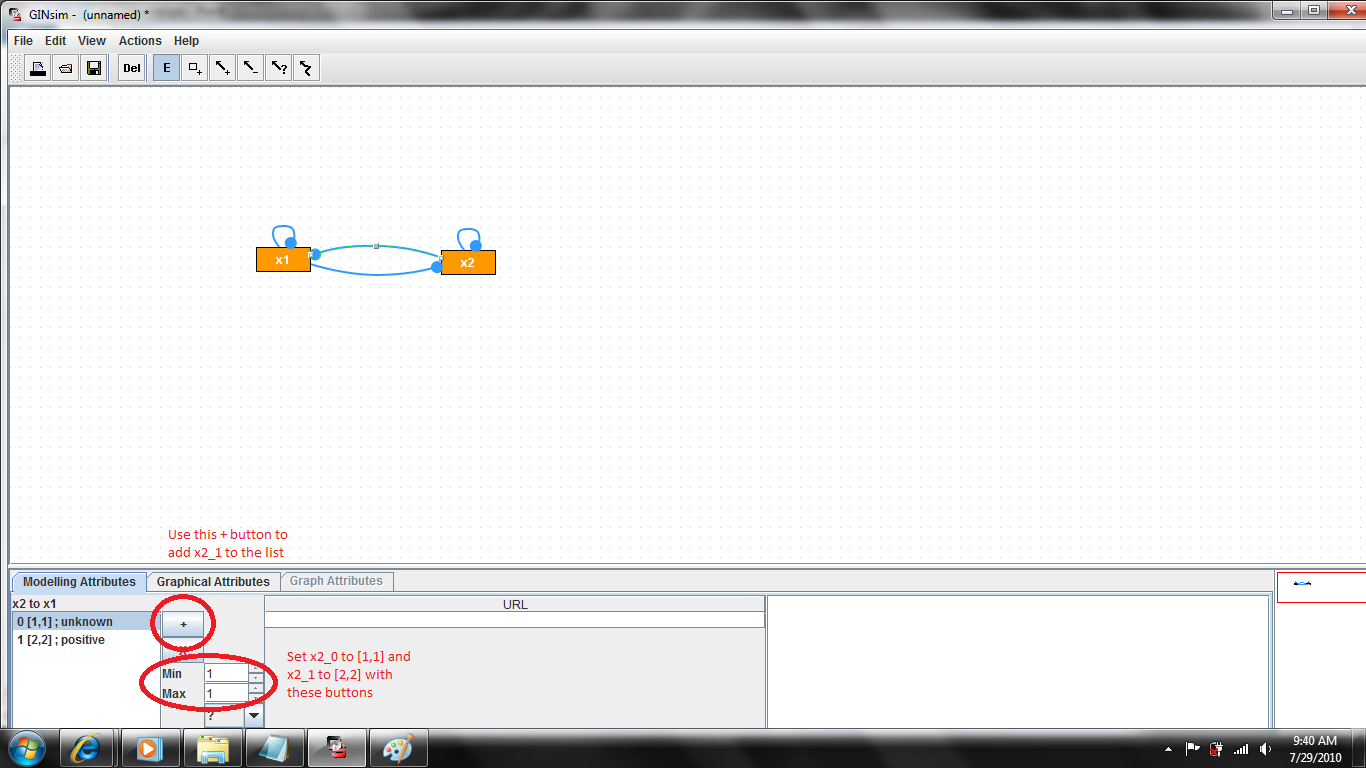
\includegraphics[scale=.43]{setedges.png}
\end{center}


 Next, for each node, do the following. For each nonzero parameter, add the corresponding nonzero values for x1, x2 and x3 
to the parameter list. If both $x_{1}$ and $x_{2}$ are nonzero, you must add them simultaneously by selecting them both with shift or control and add them to the list together. 

\begin{center}
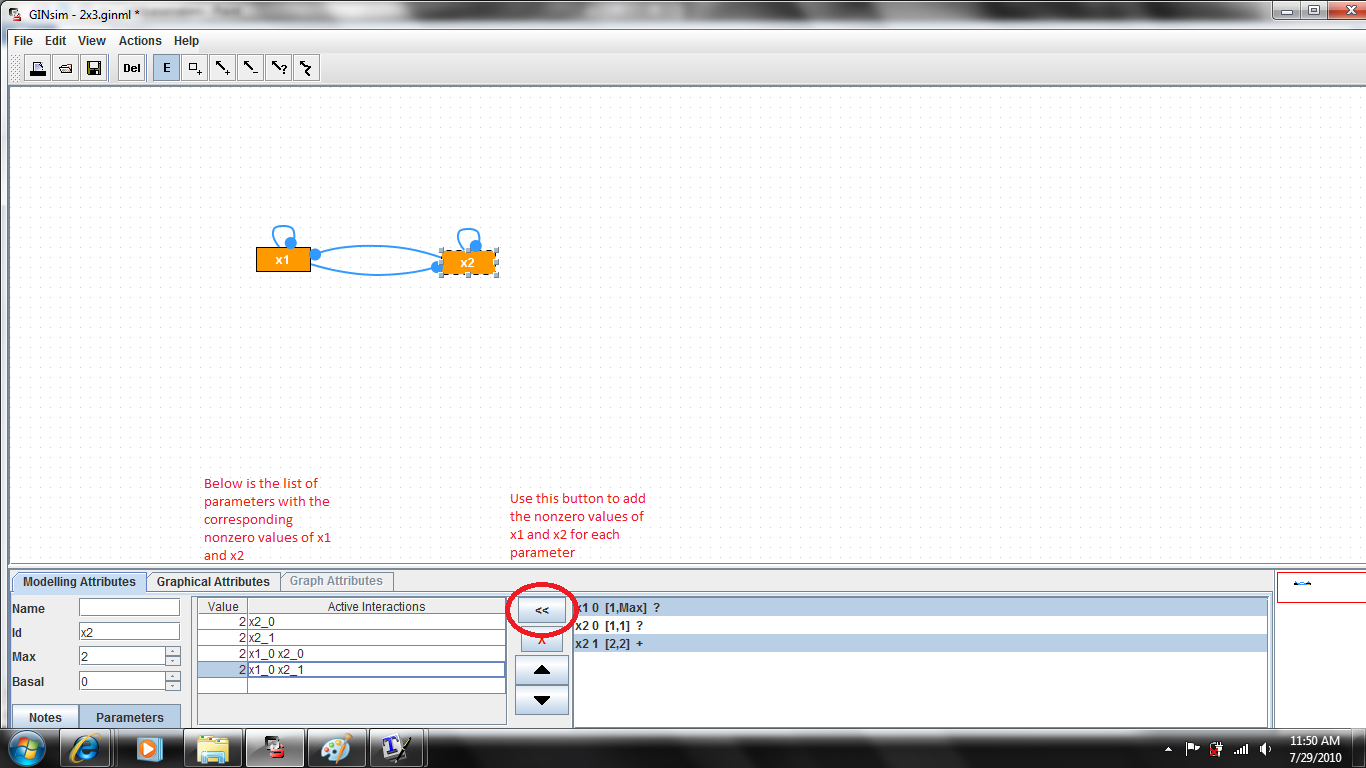
\includegraphics[scale=.43]{addparameters.png}
\end{center}

For $x_{2}$, there are four parameters, each with a value of 2. The corresponding values of $x_{1}$ and $x_{2}$ are (0,1), (0,2), (1,1) and (1,2). These are added, in that order, to the list of parameters for the model (notice the zero values are omitted). Finally, enter the value of f1 and f2 when x1 and x2 are 0 under the 
basal value.

\begin{center}
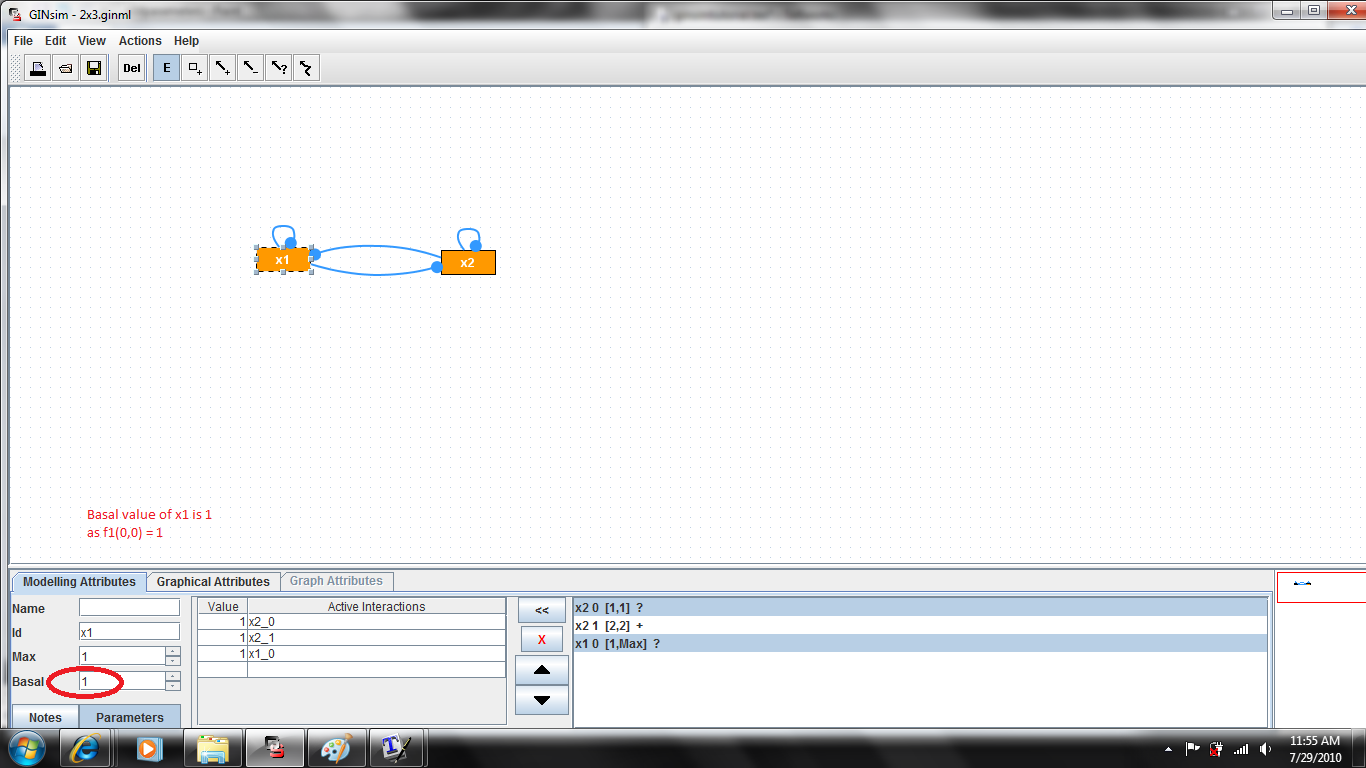
\includegraphics[scale=.43]{basal.png}
\end{center}

This is all the information necessary to construct a logical model in GINsim.

\end{document}